\documentclass{article}
\usepackage{caption, float, graphicx, subcaption}
\usepackage[dvipsnames]{xcolor}
\captionsetup[table]{skip=1em}

\title{ESE 326: Final Project}
\author{Eric Stewart \& Gabriel Minton}
\date{November 2024}


\begin{document}

\maketitle

\section{Introduction}
The maiin objective of this project involoved R's built-in dataset, Iris. Through graphical exploration and
mathematical analysis, the researchers determine
whether there are clear rules as to which of the features determine the species of a given specimen. Through 



\color{Aquamarine}


\section{Methods}

\subsection{Exploratory Analysis}


\subsection{Confidence Interval Estimate}



\subsection{Hypothesis Test}

$\sigma_1 == \sigma_2$ T-test using Sp:
\begin{equation}
	\frac{(\bar{X}_1 - \bar{X}_2) - (\mu_1 - \mu_2)}{\sqrt{{S_p}^2 \left(\frac{1}{n_1} + \frac{1}{n_2} \right)}} \sim T_{n_1 + n_2 -2}
	\label{eq:t-test_equal}
\end{equation}
\begin{equation}
	{S_p}^2 = \frac{(n_1 - 1) S_1^2 + (n_2 -1) S_2^2}{n_1 + n_2 -2}
	\label{eq:pool_sample_variance}
\end{equation}

$\sigma_1 \neq \sigma_2$ T-test using $\gamma$:
\begin{equation}
	\frac{(\bar{X}_1 - \bar{X}_2) - (\mu_1 - \mu_2)}{\sqrt{\frac{S_1^2}{n_1} + \frac{S_2^2}{n_2}}} \sim T_\gamma
	\label{eq:t-test_unequal}
\end{equation}
\begin{equation}
	\gamma = \frac{\left(\frac{S_1^2}{n_1} + \frac{S_2^2}{n_2} \right)^2}{\frac{\left(\frac{S_1^2}{n_1} \right)^2}{n_1 - 1} + \frac{\left(\frac{S_2^2}{n_2} \right)^2}{n_2 - 1}}
	\label{eq:gamma_unequal}
\end{equation}

\color{orange}
\section{Results and Observations}

\begin{figure}[H]
	\centering
	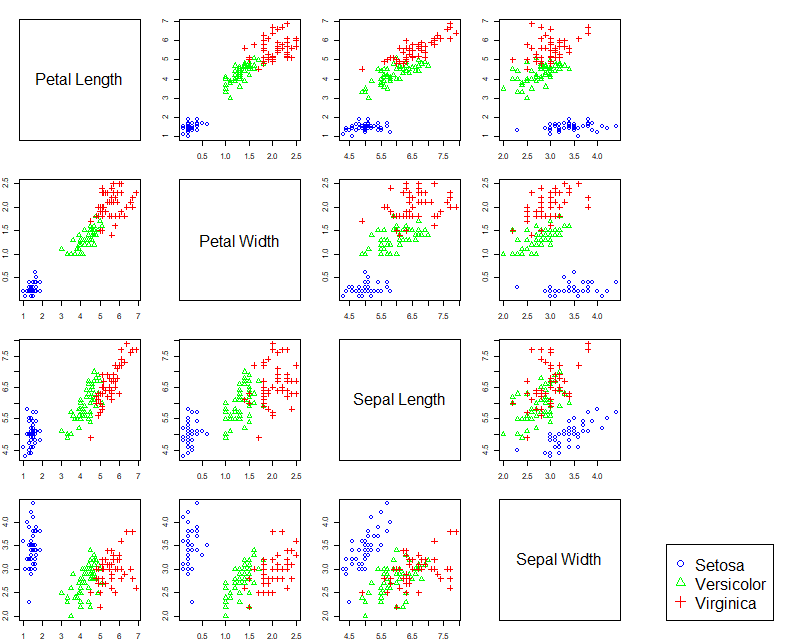
\includegraphics[width=0.75\textwidth]{iris_colored.png}
	\caption{A visualization of the Iris dataset showing scatterplots of each pair of the features.}
	\label{fig:iris_colored}
\end{figure}

% Show the feature boxplots together
\begin{figure}[H]
    \centering
    \begin{subfigure}{0.375\textwidth}
      \centering
      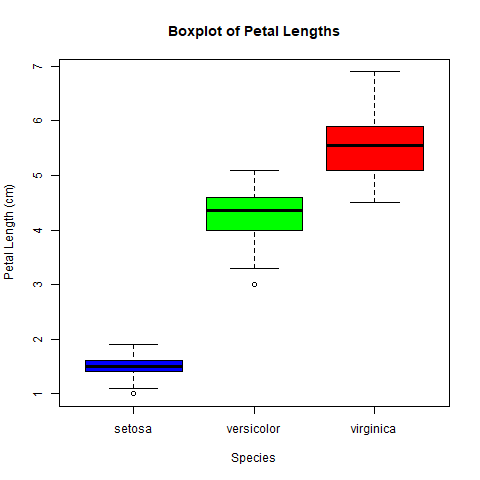
\includegraphics[width=\linewidth]{box_petal_length.png}
      \caption{Petal Lengths}
      \label{fig:feature_boxplots_A}
    \end{subfigure}%
    \begin{subfigure}{0.375\textwidth}
      \centering
      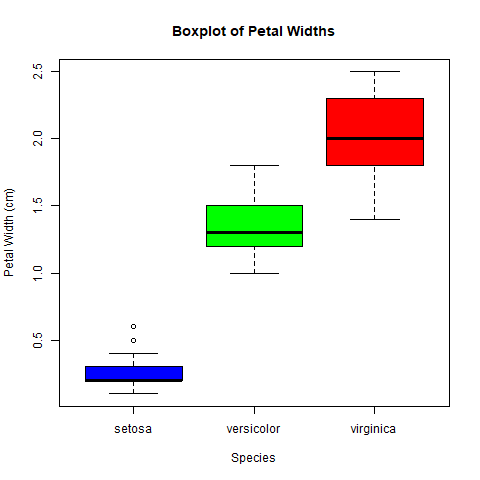
\includegraphics[width=\linewidth]{box_petal_width.png}
      \caption{Petal Widths}
      \label{fig:feature_boxplots_B}
    \end{subfigure}\\
    \begin{subfigure}{0.375\textwidth}
        \centering
        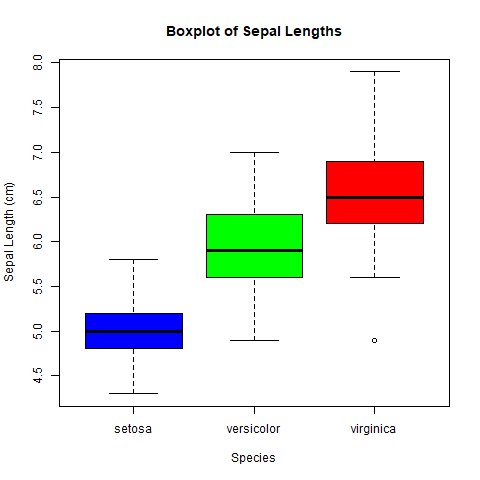
\includegraphics[width=\linewidth]{box_sepal_length.png}
        \caption{Sepal Lengths}
        \label{fig:feature_boxplots_C}
    \end{subfigure}
    \begin{subfigure}{0.375\textwidth}
        \centering
        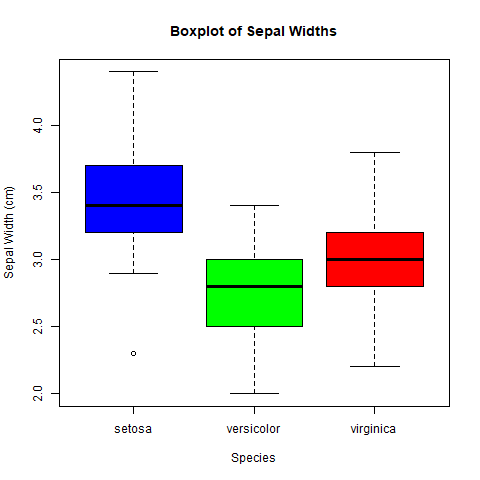
\includegraphics[width=\linewidth]{box_sepal_width.png}
        \caption{Sepal Widths}
        \label{fig:feature_boxplots_D}
    \end{subfigure}\\
    \caption{Boxplots for each of the four features.}
    \label{fig:feature_boxplots}
\end{figure}

Figure~\ref{fig:feature_boxplots_A} is petal length

% Show the histogram plot
\begin{figure}[H]
	\centering
	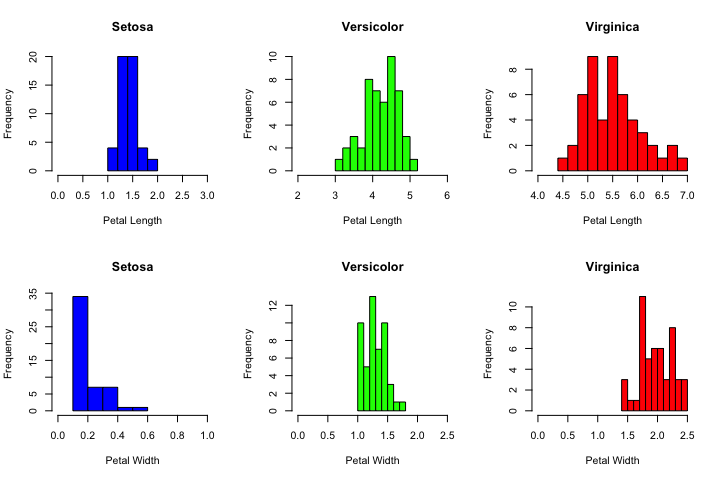
\includegraphics[width=0.75\textwidth]{hist_iris.png}
	\caption{Histograms of Petal lengths and widths for Setosa, Versicolor, and Virginica}
	\label{fig:hist_iris}
\end{figure}

\section{Conclusions}

\section{Appendix}

\subsection{R-scripts}
\subsection{Extra Figures and Tables} 



\end{document}
